\section{Model description}
\subsection{Geometry}
The \gls{SD-TMSR} design model was introduced by the \gls{CAS} as a part of  
the strategic project ``Future Advanced Nuclear Energy $-$ Thorium-based 
Molten Salt Reactor System (TMSR)" in 2011 
\cite{li_optimization_2018,jiang2012advanced,li2015analysis,li2017model}. The 
design of \gls{SD-TMSR} is inspired by \gls{MSBR} 
\cite{robertson_conceptual_1971} after some modification in the geometry to 
control the positive temperature coefficient in MSBR. The \gls{SD-TMSR} core 
geometry was described in details by Li \emph{et al.} 
\cite{li_optimization_2018}.
Figure~\ref{fig:ff} illustrates the quarter-core model configuration of the 
\gls{SD-TMSR}. The active zone is a right cylinder with height and diameter 
equal to 460 cm. Assemblies of graphite\footnote{We choose graphite density of 
$2.3$ g/cm$^3$, to validate our results against results in the literature 
\cite{li_optimization_2018,nuttin2005potential}.} hexagonal prisms fill the 
core. The side length of the graphite hexagonal prism was optimized in 
\cite{li_optimization_2018} and found to be 7.5 cm. The liquid fuel circulates 
continuously through the fuel channels that pierces the graphite hexagonal 
prisms. The core is divided into two different zones to enhance 
Th/$^{233}$U breeding performance. The radius of the fuel channels in the 
outer and inner zone are 5 and 3.5 cm, respectively. The axial and radial 
graphite reflectors surround the core to minimize neutron leakage and 
maximize flux in the core. The reflectors are surrounded by B${_4}$C cylinder 
that acts as a radiation shielding. The \gls{SD-TMSR} pressure vessel holds 
the fuel salt, graphite elements, reflector, shielding, intermediate heat 
exchanger (IHX) and made of Ni-based (hastelloy N) alloy. The main 
characteristics of the \gls{SD-TMSR} are listed in Table~\ref{tab:table1}.

\begin{figure} % replace 't' with 'b' to \centering [hbp!]
	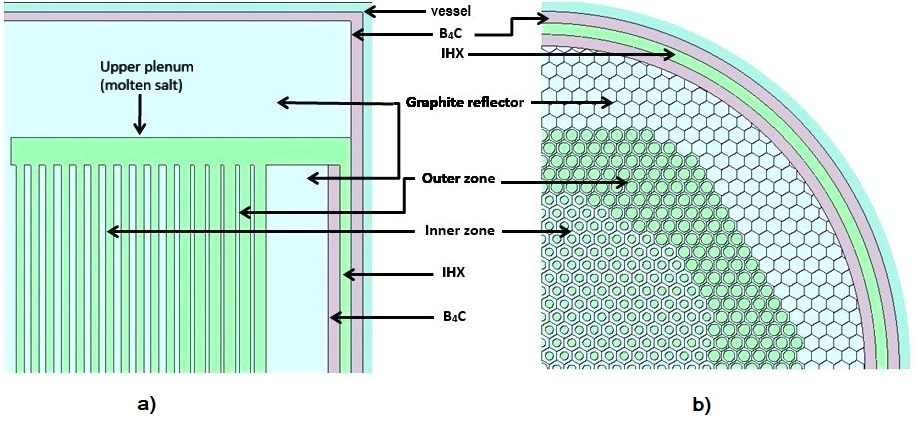
\includegraphics[width=\textwidth]{ff.png}
	\caption{$XZ$ (a) and $XY$ (b) section of the quarter-core model of the 
	SD-TMSR.}
	\label{fig:ff}
\end{figure}

\begin{table}  %[!ht]
	\caption{The main characteristics of the SD-TMSR \cite{li_optimization_2018}}
	\vspace{0.1in}
	\begin{tabularx}{\textwidth}{l | l}
		\hline
		Thermal power, MW$_{th}$          				&  2,250  \\ 
		Fuel salt components                            & LiF-BeF$_2$-(\gls{HM})F$_4$ \\
		Fuel composition, mole\%                        & 70-17.5-12.5    \\
		$^7$Li enrichment, \%        				& 99.995   \\
		Fuel temperature, K 							& 900  \\
		Fuel density at 900 K, g/cm$^3$		  		& 3.3 \\
		Fuel dilatation coefficient, g/(cm$^3$ $.$K)  &  -6.7$\times$10$^{-4}$ \\
		Graphite density, g/cm$^3$             	    & 2.3	\\  
		B$_4$C density, g/cm$^3$					& 2.52  \\
		$^{10}$B enrichment, \%						&  18.4  \\
		Core diameter, cm								& 460  \\
		Core height, cm									& 460  \\
		Side length of the graphite hexagonal prism, cm   & 7.5 \\
		Inner radius, cm							& 3.5  \\
		Outer radius, cm							& 5  \\
		Ratio of molten salt and graphite in the inner zone	&  0.357  \\
		Ratio of molten salt and graphite in the outer zone &  1.162  \\
		Fuel volume, m$^3$  &	52.9 \\
		\hline
	\end{tabularx}
	\label{tab:table1}
\end{table}
%%%%%%%%%%%%%%%%%%%%%%%%%%%%%%%%%%%%%%%%

%\begin{figure}[t!] % replace 't' with 'b' to \centering
%	\hspace{+0.65in}
%	\includegraphics[width=\textwidth]{core.png}
%	\caption{Plan view of SD-TMSR core.}
%	\label{fig:core}
%\end{figure}

\subsection{Fuel composition}
The general composition of the liquid fuel salt in this work is 70LiF - 
17.5BeF$_2$ - 12.5(HM)F$_4$ mole\%, where HM is the heavy metal (misture of 
thorium and other actinides). The aim of this paper is to simulate the  
operation of \gls{SD-TMSR} for 60 years with different startup fissile 
compositions and without any external feed of fissile $^{233}$U which we 
assumed is unavailable. For that reason, five different types of initial 
fissile materials based on \gls{LEU}, Pu, and \gls{TRU} from LWR SF were 
considered:
\begin{enumerate}[label=(\alph*)]
	\item low-enriched uranium (LEU) (19.79\%);
	\item Pu mixed with \gls{LEU} (19.79\%);
	\item Pu reactor-grade \cite{marka1993explosive};
	\item transuranic (TRU) elements from LWR SF \cite{de2000scenarios};
	\item $^{233}$U for comparison purpose \cite{ashraf2019whole_core}.
\end{enumerate}

The reactor-grade plutonium and \gls{TRU} composition are summarized in 
Table~\ref{tab:table2} and ~\ref{tab:table3}, respectively.

\begin{table}  %[!ht]
	\caption{Reactor-grade plutonium vector \cite{marka1993explosive}}
	\vspace{0.1in}
	\begin{tabularx}{\textwidth}{s s s s s}
		\hline
		$^{238}$Pu & $^{239}$Pu & $^{240}$Pu & $^{241}$Pu & $^{242}$Pu \\
		\hline
		 1.3&60.3&24.3&9.1&5 \\
		\hline
	\end{tabularx}
	\label{tab:table2}
\end{table}

\begin{table}  %[!ht]
	\caption{\gls{TRU} vector (\%) \cite{de2000scenarios}}
	\vspace{0.1in}
	\begin{tabularx}{\textwidth}{s s s s s s s s s s}
		\hline
		$^{237}$Np&$^{238}$Pu & $^{239}$Pu & $^{240}$Pu & $^{241}$Pu & $^{242}$Pu&$^{241}$Am &$^{243}$Am&$^{244}$Cm &$^{245}$Cm\\
		\hline
		6.3&2.7&45.9&21.5&10.7&6.7&3.4&1.9&0.8&0.1 \\
		\hline
	\end{tabularx}
	\label{tab:table3}
\end{table}

For reactor-grade plutonium case, the composition was taken for plutonium 
recovered from the spent fuel composition of commercial \gls{PWR} with the 
average discharge burnup $33$ $GWd/t$ and after $10$ years of cooling before 
reprocessing \cite{oecd1989probabilistic,marka1993explosive}. Similarly, the 
isotopic compositions of \gls{TRU} was taken for the SF of UOX \gls{PWR} 
(after one use, no multi-recycling) with the average discharge $60$ 
$GWd/t$ burnup, and after $5$ years of cooling \cite{de2000scenarios}. 
The molar composition of startup fuel for all five cases is listed in 
Table~\ref{tab:table4}. Meanwhile, the corresponding initial nuclei 
inventories with different types of fuel are summarized in 
Table~\ref{tab:table5}.
\begin{table}  %[!ht]
	\caption{Composition of startup fuel (mole\%)}
	\vspace{0.1in}
	\begin{tabularx}{\textwidth}{p{0.16\textwidth} X p{0.17\textwidth} 
	p{0.14\textwidth} X X}
		\hline
		Fuel salt component& \gls{LEU} (19.79\%) & Pu+enriched U (19.79wt\%) 
		& Pu reactor-grade & \gls{TRU}& $^{233}$U \\
		\hline
		LiF&70&70&70&70&70\\
		BeF$_2$&17.5&17.5&17.5&17.5&17.5\\
		ThF$_4$&8.25&7.5&10.75&	8.65&12.3		\\
		UF$_4$&4.25&4.75&&&	0.2		\\
		PuF$_3$&&0.25&1.75&&		\\
		(TRU)F$_3$&&&	&3.85	&\\
		\hline
	\end{tabularx}
	\label{tab:table4}
\end{table}

\begin{table}  %[!ht]
	\caption{Initial nuclei inventories (in grams) of the SD-TMSR with different types of fuel.}
	\vspace{0.1in}
	\begin{tabularx}{\textwidth}{s s s s s s}
		\hline
		\vspace{0.1in}
		Molecule& \gls{LEU} (19.79\%) & Pu mixed with enriched U (19.79\%) & Pu reactor-grade & \gls{TRU}& $^{233}$U \\
		\hline
		$^{232}$Th       &6.24E+07 & 4.67E+07 &   6.75E+07			& 5.44E+07	& 7.69E+07    \\ 
		$^{233}$U        &         & &        &       &  1.30E+06 \\
		$^{235}$U        & 3.17E+06 &6.01E+06	&            &   & \\
		$^{238}$U      	 &1.28E+07  &2.43E+07 &	&  &\\
		$^{237}$Np	  	 &         && &1.58E+06	&    \\
		$^{238}$Pu	  	 &         &1.60E+04	& 1.13E+05 & 6.78E+05	&   \\
		$^{239}$Pu       &         &9.59E+05&6.76E+06& 1.15E+07&    \\
		$^{240}$Pu       &         &3.99E+05& 2.82E+06&5.40E+06&  	\\  
		$^{241}$Pu		 &         &1.60E+05&1.13E+06&2.69E+06&   \\
		$^{242}$Pu		 &         &6.39E+04	&4.51E+05	& 1.68E+06& \\
		$^{241}$Am		 &         &&& 8.53E+05 & \\
		$^{242}$Am		 &         &&&  &\\
		$^{243}$Am       &        & &&4.77E+05&\\
		$^{244}$Cm		 &        & &&2.01E+05&  \\
		$^{245}$Cm		 &        & &&			2.51E+04	&   \\
		&         &&		&		&\\
		Total mass \\of HM without $^{232}$Th	& 1.60E+07& 3.20E+07&1.13E+07&  2.51E+07&   1.30E+06  \\
		\hline
	\end{tabularx}
\label{tab:table5}
\end{table}


\section{Methodology and tools}

Simulation of Liquid-fueled Molten Salt Reactor (MSR) systems requires 
computational software that must support online fuel salt reprocessing and 
refueling \cite{serp2014molten}. In this work, SERPENT-2 version 2.1.31 
beta\footnote{SERPENT-2 is a 3D continuous energy Monte Carlo neutron 
transport and burnup code.} \cite{leppanen2014serpent} is used to simulate the 
full-core of the SD-TMSR with different types of initial fuel. The extension 
of SERPENT accounts for continuous online reprocessing and refueling 
\cite{aufiero2013extended}. ENDF-VII.0 cross-section library was used for all 
calculations in this work. The results demonstrate full-core runs of 
$1.25\times 10^7$ neutron history per depletion step. The full burnup time of 
the SD-TMSR was 60 years with statistical error in $k_{eff}$ equal to $\pm$ 
$36$ $pcm$. The online extraction of \gls{FPs} and other neutron absorbers 
provides many benefits for MSRs. For example, it would reduce the initial 
fissile material inventory required to achieve criticality and improve the 
breeding ratio. Figure~\ref{fig:flow} shows a flow chart of the calculation 
steps. 

\begin{figure}[t!] % replace 't' with 'b' to \centering
	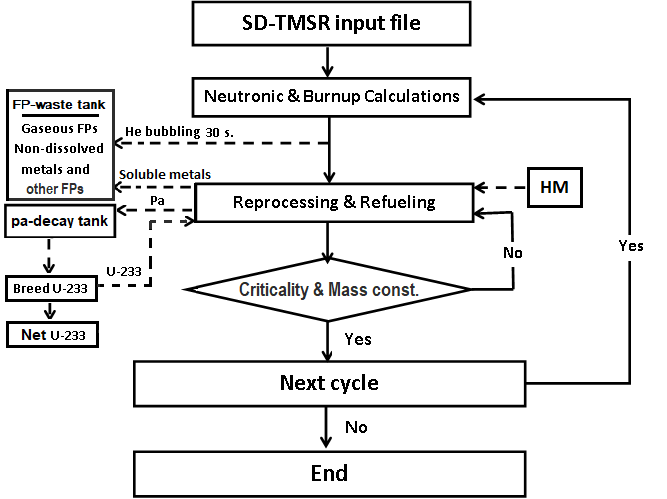
\includegraphics[width=\textwidth]{flowch.png}
	\caption{Flow chart of the calculation procedures.}
	\label{fig:flow}
\end{figure}

As shown in Figure~\ref{fig:flow}, after launched the input file, an advanced 
matrix exponential solution based on the Chebyshev Rational Approximation 
Method (CRAM) \cite{isotalo2016improving} used to solve the Bateman equation. 
Then, the system extracted gaseous \gls{FPs} and other materials 
(non-dissolved metals, lanthanides, and soluble metals except Pu) with 
suitable removal rate\footnote{The extraction rate depends on the type of 
poison and its impact on the neutron
economy.}. This can be done by set the 
flow rate of gaseous \gls{FPs} and other materials from the fuel to the 
\texttt{FP-waste tank}\footnote{An imaginary tank used to store the gaseous 
\gls{FPs} and the other materials (non-dissolved metals, lanthanides, and 
soluble metals except protactinium).}. Specifically, protactinium was removed 
from the fuel with a certain flow rate into the external tank, 
\texttt{pa-decay tank}\footnote{An imaginary tank used to store protactinium 
extracted from the core.}, to decay and produce $^{233}$U\footnote{The 
$^{233}$Pa is removed and left to decay into $^{233}$U with $\tau_{1/2}$ 
$\approx$ $27$ $d$.}. The produced $^{233}$U is used as a fresh fissile fuel 
and the residual $^{233}$U is the net production of $^{233}$U. The MSR burnup 
routine provided by SERPENT-2 allows changes the flow rates ($mflow$) of the 
isotopes during reactor operation \cite{aufiero2013extended}. The mass of the 
fissile and fertile materials needed to achieve criticality is calculated at 
the end of the cycle. Then, this mass is added to the core at the beginning of 
the cycle by a certain flow rate.

\section{Feed and extraction rates}
In the present work, two different feed mechanisms are used. The first 
mechanism allows continuous feed flow of thorium from Th stockpile, and 
$^{233}$U from \texttt{pa-decay tank}. In contrast, the second mechanism 
continuously injects Heavy Metal (HM) (excluding Th) and simultaneously feeds  
all or part of produced $^{233}$U from \texttt{Pa-decay tank}. The fission 
products act as poisons in the MSRs; they negatively impacting the reactivity. 
Therefore, \gls{FPs} must be extracted during reactor operation. Consider 
$T_{r}$ as the time during which the total fuel salt is reprocessed and 
$dN_{e}$ as the amount of particular element $e$ with inventory $N_{e}$ that 
the \gls{MSR} extracts during time $dt$; thus \cite{nuttin2005potential}

\begin{equation}
\label{Equ:1}
\dfrac{dN_{e}}{dt} = N_{e}\dfrac{\varepsilon_{e}}{T_{r}},	
\end{equation}

where $\varepsilon_{e}$ is the removal efficiency. Equation \ref{Equ:1} gives 
the removal constant $\lambda_{e}$ $[s^{-1}]$ (the rate at which the material 
is removed), where $\lambda_{e}=\varepsilon_{e}/T_{r}$. The removal constant 
$\lambda_{e}$ of gaseous and other fission products is precisely calculated 
and summarized in Table~\ref{tab:table6}. The effective reprocessing time for 
the gaseous \gls{FPs} and non-dissolved metals was set to 30 seconds (removal 
constant $\lambda_{e}$ = $-0.0333$ $s^{-1}$), because such elements must be 
extracted promptly and continuously via gas removal system. In contrast, 
extracting the soluble \gls{FPs}, lanthanides, and protactinium can be done by 
the chemical reprocessing (i.e. fluorination and reduction reaction). 
Therefore, the system reprocesses a specific amount of fuel salt daily. In the 
present work, the effective extraction time for soluble \gls{FPs} is 
$\approx$10.59 days ($\lambda_{e}$ = $-1.092\times10^{-6}$ $s^{-1}$), which is 
equivalent to 5 m$^3$/d of chemical reprocessing rate 
\cite{nuttin2005potential,li_optimization_2018}. The effective feed rates of 
the heavy metals (HM) are changed during reactor operation to conserve the 
total fuel mass and criticality.


\begin{table}[ht!]
	\centering
	\caption{The reprocessing table.} 
	\vspace{1ex}
	\begin{tabularx}{\textwidth}{|p{2.3cm}|p{4.5cm}|s|p{2cm}|}
			\hline
			\textbf{Reprocessing group}  & \textbf{Element} & \textbf{Reproc- essing time} & \textbf{Removal constant} $\lambda_{e}$ $[s^{-1}]$ \\
			\hline
			Gaseous \gls{FPs} and non-dissolved metals  &  H, He, N, O, Ne, Ar, Kr, Nb, Mo, Tc, Ru, Rh, Pd, Ag, Sb, Te, Xe, Lu, Hf, Ta, W, Re, Os, Ir, Pt, Au and Rn.		&	30s	&  -3.333E-02 \\
			\hline
			Lanthanides and other soluble \gls{FPs}     & 
			Zn, Ga, Ge, As, Se, Br, Rb, Sr, Y, Zr, Cd, In, Sn, I, Cs, Ba, La, Ce, Pr, Nd, Pm, Sm, Eu, Gd, Tb, Dy, Ho, Er, Tm and Yb. & 10.599 d (5 m$^3$/d) &  -1.092E-06 \\
			\hline
			Protactinium   & Pa  &  10.599 d (5 m$^3$/d)  &  -1.092E-06 \\
			\hline
	\end{tabularx}
	\label{tab:table6}
\end{table}

%\begin{table}[ht!]
%	\centering
%	\caption{The refueling table.} 
%	\vspace{1ex}
%	\begin{tabularx}{\textwidth}{|p{1.5cm}|b|p{1.9cm}|}
%		\hline
%		\textbf{Nuclide} & \textbf{Feed rate} & \textbf{Feed constant$^{\star}$} $\lambda_{e}$ $[s^{-1}]$ \\
%		\hline
%		$^{232}$Th        &  1.842 [Kg/day], first 90 [d] & 1.500E-09 \\
%		&  2.511 [Kg/day], from 90 to 1550 [d] & 		2.045E-09 \\
%		&  2.456 [Kg/day], from 1550 to 3010 [d] & 		2.000E-09 \\
%		&  2.321 [Kg/day], from 3010 to 5930 [d]& 		1.890E-09	\\
%		&  2.241 [Kg/day], from 5930 to 7390 [d] &		1.825E-09	\\
%		&  2.186 [Kg/day], from 7390 to 12500 [d] &		1.780E-09	\\
%		&  2.118 [Kg/day], from 12500 to 15420 [d] &	1.725E-09	\\
%		&  2.136 [Kg/day], from 15420 to 18340 [d]&		1.740E-09		\\
%		&  2.063 [Kg/day], from 18340 to 21900 [d]&		1.680E-09	 \\ 
%		\hline
%		$^{233}$U & 2.619 [Kg/day], first 90 [d]	&   6.400E-09  \\
%		& 2.009 [Kg/day],  form 90 to 1550 [d] &	4.910E-09 \\
%		& 1.944 [Kg/day], from 1550 to 3010 [d] &	4.750E-09 \\
%		& 1.826 [Kg/day],  from 3010 to 5930 [d] &	4.460E-09 \\
%		& 1.811 [Kg/day],  from 5930 to 7390[d] &	4.425E-09 \\
%		& 1.744 [Kg/day], from 7390 to 12500 [d] &	4.260E-09 \\
%		& 1.699 [Kg/day], from 12500 to 18340 [d]	& 4.150E-09 \\
%		& 1.657 [Kg/day], from 18340 to 21900 [d]	& 4.050E-09 \\
%		\hline
%	\end{tabularx}
%	\begin{tablenotes}
%		\small
%		\item  $^{\star}$ Feed constant is the mass fraction of fissile nuclide ($^{232}$Th or $^{233}$U) transferred from the external storage to the core per second.
%	\end{tablenotes}
%	\label{tab:table3}
%\end{table}	